


\begin{document}

This report describes the design, implementation and test of an LED (light emmitting diode) driver. 

\noindent This report describes design, implementation and test of an LED driver comprised of a ring oscillator, Schmitt trigger, and a current driver. The ring oscillator is comprised of complementary metal oxide semiconducting field effect transistors (CMOS) inverters connected in series. Figure \ref{fig:blockdiagram2} demonstrates where in the optical uplink project the LED driver is placed. 



\begin{figure}[H]
    \centering
    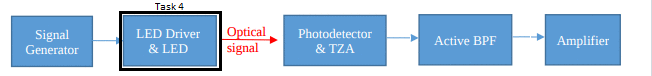
\includegraphics[width=.9\textwidth ]{Introduction/Block_Diagram_MFBP.png}
    \caption{Block diagram for optical uplink \cite{b1}}
    \label{fig:blockdiagram2}
\end{figure}

The specifications for this lab are summarized in Table \ref{tab:specifications}.

\begin{table}[H]
	\centering
	\caption{LED driver specifications}
	\label{tab:specifications}
	\begin{tabular}{|l|l|}
		\hline
		Specifications & Required       \\ \hline
		Frequency      & 20kHz$\pm 5\%$ \\ \hline
		Duty-cycle     & 50\%           \\ \hline
		Amplitude      & $\geq$100mA    \\ \hline
	\end{tabular}
\end{table}


The LED driver circuit supplies the LED with a controlled current. A signal conditioner takes the output from a ring oscillator and creates a 50\% duty-cycle square wave. The square wave is then in turn recieved by a current driver. The current driver creates a sufficiently large current in order to operate the LED.  A voltage driven output to light the LED is not used due to increased sensitivity from temperature change. 



\end{document}